\documentclass[aspectratio=169]{beamer}
% \usetheme{Madrid}

\usefonttheme{serif}
\setbeamercolor{normal text}{fg=black}

% Make all structural text black (titles, sections, etc.)
\setbeamercolor{structure}{fg=black}

% Frame titles (top title)
\setbeamercolor{frametitle}{fg=black}

% Figure caption ("Figure:")
\setbeamercolor{caption name}{fg=black}
\setbeamercolor{caption}{fg=black}

% Section titles in footer/header
\setbeamercolor{section in head/foot}{fg=black}

% Just in case
\setbeamercolor{title}{fg=black}


% --- Theme setup (minimal) ---
\usetheme{default}
\useoutertheme{default}
\useinnertheme{default}

% Remove navigation symbols
\setbeamertemplate{navigation symbols}{}

% Define your red
% \definecolor{myred}{RGB}{225,120,120}
\definecolor{myred}{RGB}{115,0,10}


\usepackage{color} % color added for editing
\newcommand{\bl}[1]{\textcolor[rgb]{0.00,0.00,1.00}{#1}}
\newcommand{\gr}[1]{\textcolor[rgb]{0.00,0.50,0.00}{#1}}
\newcommand{\rd}[1]{\textcolor[rgb]{0.75,0.00,0.00}{#1}}
\newcommand{\tl}[1]{\textcolor[rgb]{0,0.6,0.60}{#1}}

\usepackage{booktabs}
\usepackage{bm}
\usepackage{mdframed}
\usepackage{xcolor}

% --- Custom footline ---
\setbeamertemplate{footline}{
\leavevmode

% Thin red line (moved to TOP)
\begin{beamercolorbox}[wd=\paperwidth,ht=0.1ex]{}
\color{myred}\rule{\paperwidth}{0.1ex}
\end{beamercolorbox}

\hbox{
\begin{beamercolorbox}[wd=\paperwidth,ht=2.5ex,dp=1ex]{}
\hspace{1em}
\insertsection
\hfill
\insertframenumber{} / \inserttotalframenumber
\hspace{1em}
\end{beamercolorbox}
}
}

% Remove headline entirely
\setbeamertemplate{headline}{}

% Optional: clean fonts
\setbeamerfont{footline}{size=\small}







\title{Chapter~5~Regression-Based Classification}
\author{Austin R.J. Downey}
\date{}

\begin{document}

\section{Machine Learning for Engineering Problem Solving}
\frame{\titlepage}


\section{Chapter~5~Regression-Based Classification}

\section{3.1~Logistic Regression}


\begin{frame}{Regression-Based Classification}
\begin{columns}

\column{0.42\textwidth}

Regression models can often be adapted for classification.

\vspace{0.5em}

Examples:
\begin{itemize}
\item Linear Regression $\rightarrow$ Logistic Regression
\item Logistic Regression $\rightarrow$ Softmax Regression
\end{itemize}

\vspace{0.5em}

Advantages:
\begin{itemize}
\item Interpretable models
\item Familiar hyperparameters
\item Probabilistic predictions
\end{itemize}

\column{0.58\textwidth}
\centering
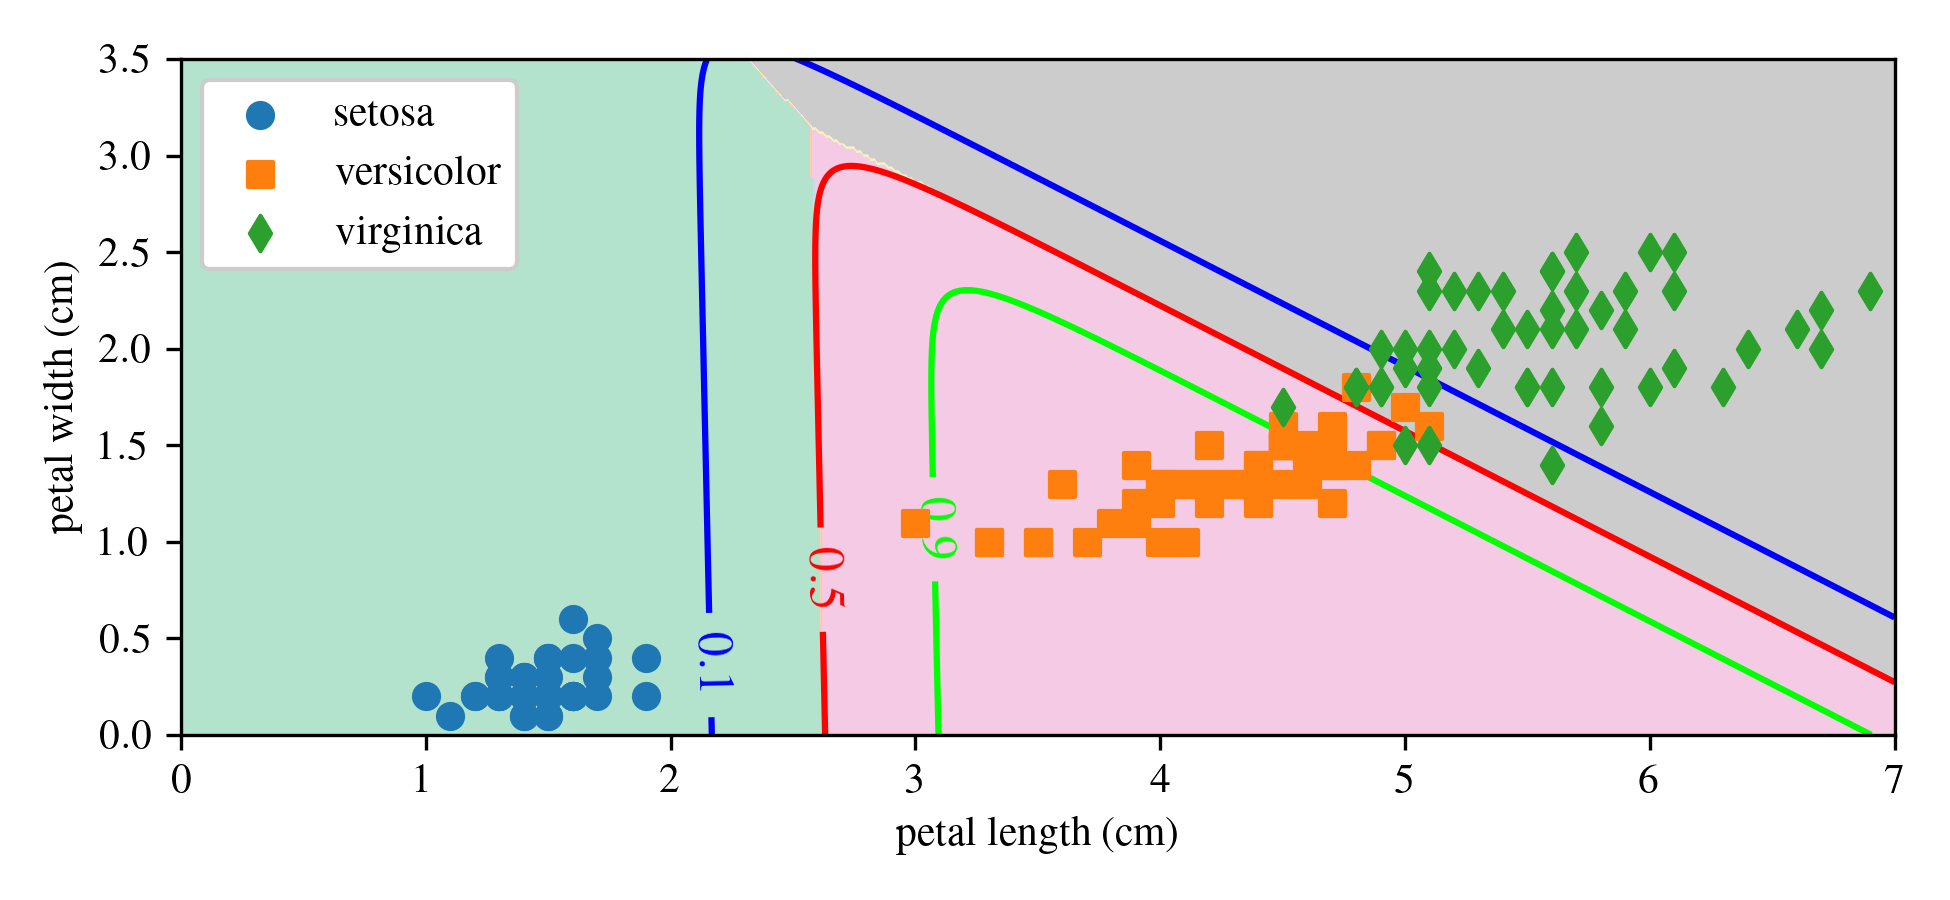
\includegraphics[width=\textwidth]
{../figures/Softmax_classification.png}

\vspace{0.3em}
{\small Classification regions for the three Iris species.}

\end{columns}
\end{frame}

%------------------------------------------------

\begin{frame}{Logistic Regression}

Logistic Regression estimates the probability that an input belongs to a class.

\vspace{0.5em}

Predicted probability:

\[
\hat{p}
=
h_\theta(X)
=
\sigma(\bm{\theta}^{\top}X)
\]

\vspace{0.5em}

Classification rule:

\[
\hat{y}
=
\begin{cases}
0 & \hat{p}<0.5\\
1 & \hat{p}\ge 0.5
\end{cases}
\]

\vspace{0.5em}

\begin{itemize}
\item Binary classifier
\item Output is a probability
\item Threshold typically set to 50\%
\end{itemize}

\end{frame}

%------------------------------------------------

\begin{frame}{The Sigmoid Function}
\begin{columns}

\column{0.45\textwidth}

The sigmoid function maps any real number to the interval $(0,1)$:

:contentReference[oaicite:0]{index=0}

\vspace{0.5em}

\begin{itemize}
\item S-shaped curve
\item Converts scores into probabilities
\item Central component of Logistic Regression
\end{itemize}

\column{0.55\textwidth}
\centering
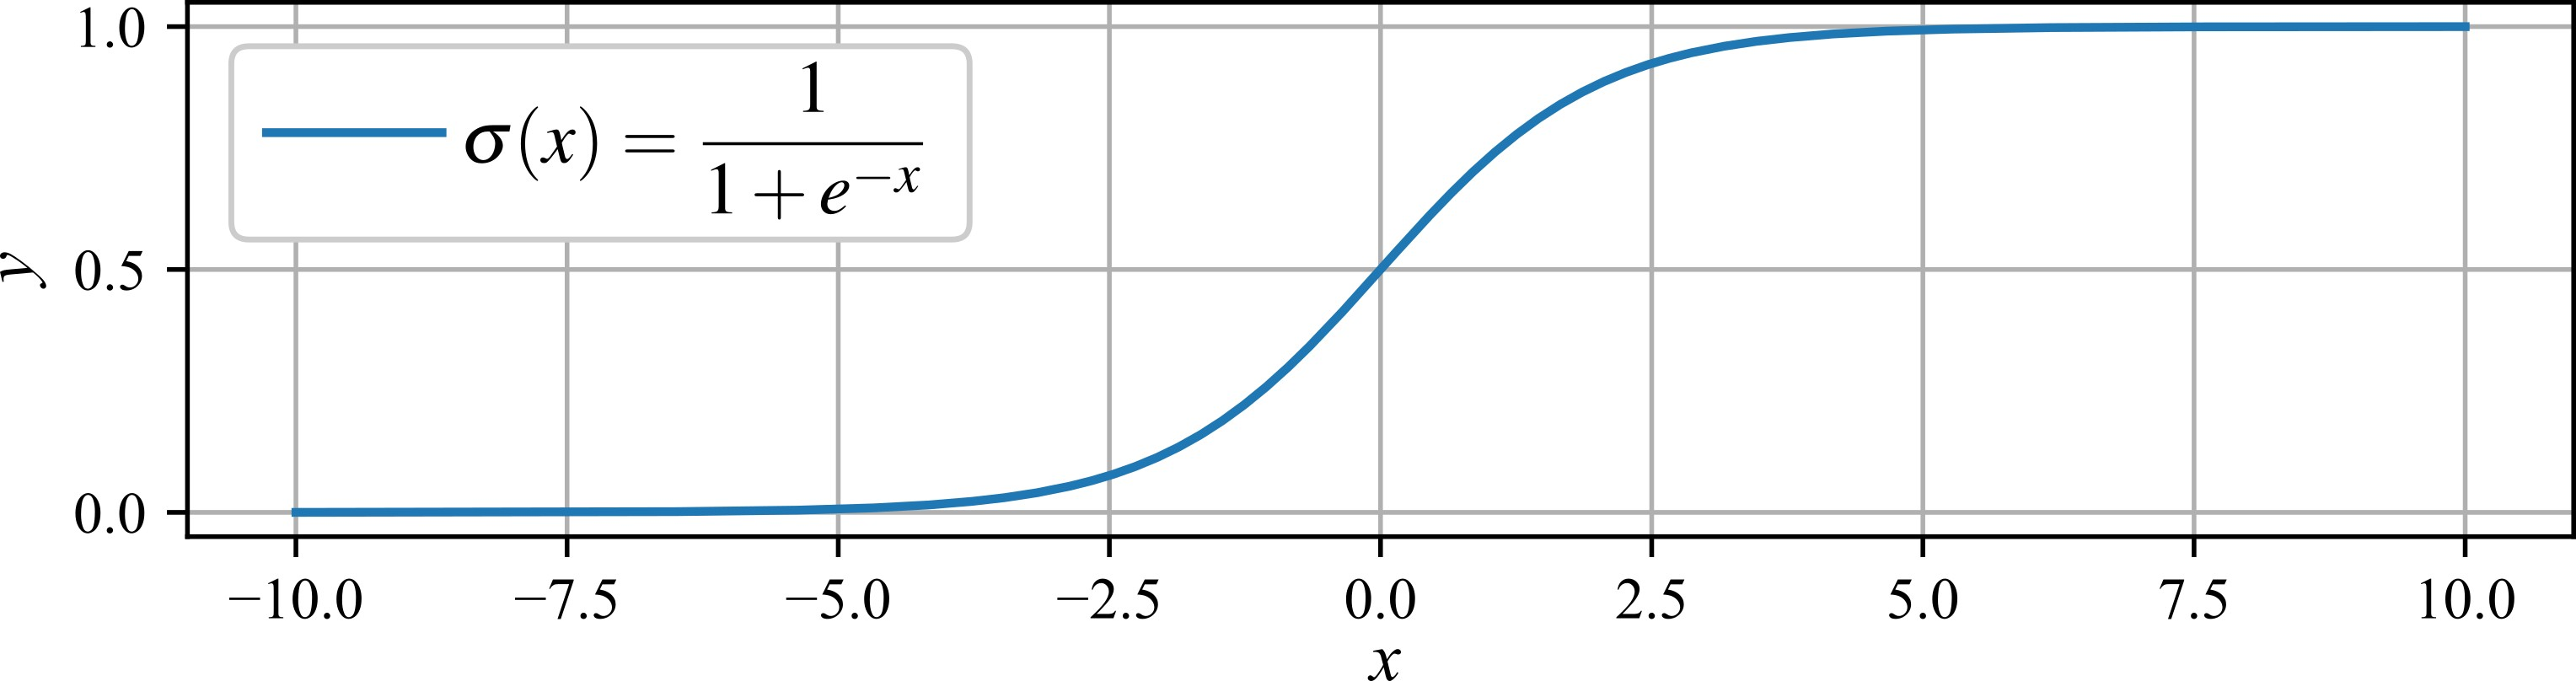
\includegraphics[width=\textwidth]{../figures/sigmoid_function}

\vspace{0.3em}
{\small Sigmoid function.}

\end{columns}
\end{frame}

%------------------------------------------------

\begin{frame}{Classification Cost Function}
\begin{columns}

\column{0.48\textwidth}

Training Logistic Regression requires a cost function that:

\begin{itemize}
\item Rewards correct predictions
\item Penalizes incorrect predictions
\item Produces probabilities near:
\begin{itemize}
\item 1 for positive examples
\item 0 for negative examples
\end{itemize}
\end{itemize}

\vspace{0.5em}

Observations:
\begin{itemize}
\item Large penalty when a confident prediction is wrong
\item Small penalty when a confident prediction is correct
\end{itemize}

\column{0.52\textwidth}
\centering
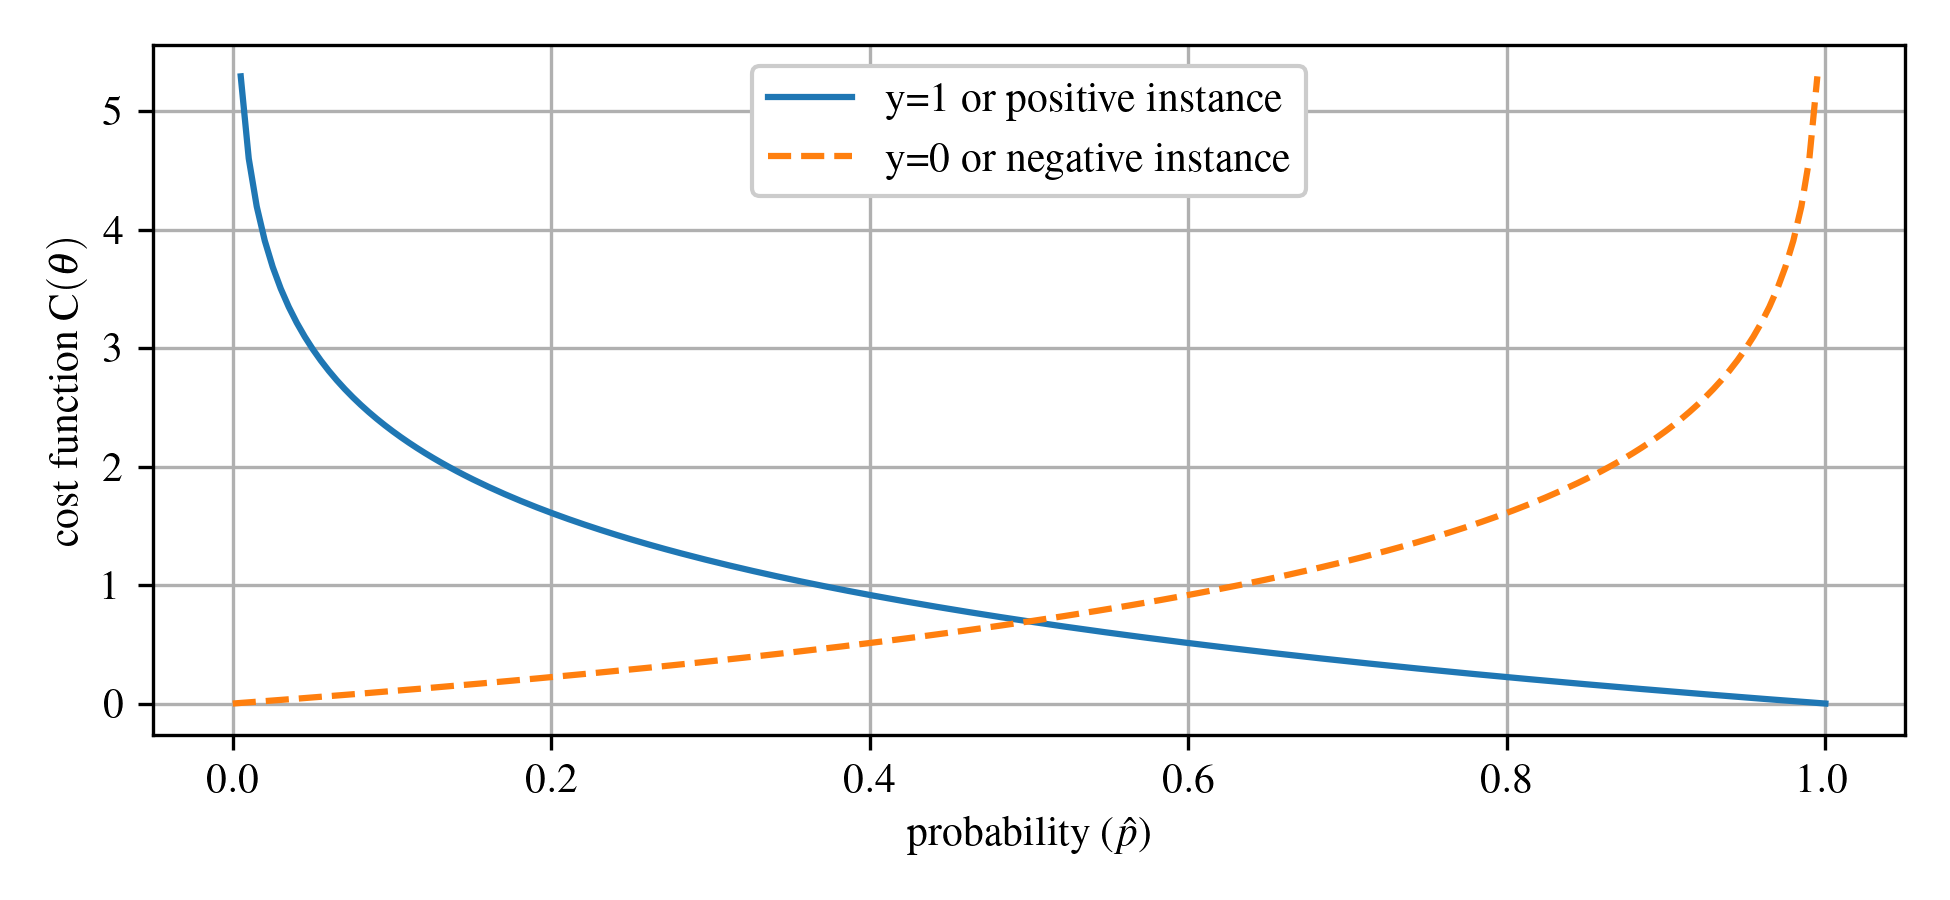
\includegraphics[width=\textwidth]
{../figures/Logistic_Regression_cost_function.png}

\vspace{0.3em}
{\small Classification cost function.}

\end{columns}
\end{frame}

%------------------------------------------------

\begin{frame}{Training Logistic Regression}

Cost for a single sample:

\[
C(\theta)=
\begin{cases}
-\log(\hat{p}) & y=1 \\
-\log(1-\hat{p}) & y=0
\end{cases}
\]

\vspace{0.5em}

Overall cost (log-loss):

\[
J(\theta)
=
-\frac{1}{m}
\sum_{i=1}^{m}
\Big[
y^{(i)}\log(\hat{p}^{(i)})
+
(1-y^{(i)})
\log(1-\hat{p}^{(i)})
\Big]
\]

\vspace{0.5em}

\begin{itemize}
\item No closed-form solution
\item Train using Gradient Descent
\item Convex cost function
\item Guaranteed global minimum
\end{itemize}

\end{frame}

%------------------------------------------------


\begin{frame}{Data: Iris Flower Dataset}
\begin{columns}

\column{0.48\textwidth}

The Iris dataset contains measurements from:

\begin{itemize}
\item 150 flowers
\item 3 species:
\begin{itemize}
\item Iris-Setosa
\item Iris-Versicolor
\item Iris-Virginica
\end{itemize}
\end{itemize}

\vspace{0.5em}

Features:
\begin{itemize}
\item Sepal length
\item Sepal width
\item Petal length
\item Petal width
\end{itemize}

\vspace{0.5em}

A classic classification dataset.

\column{0.52\textwidth}
\centering
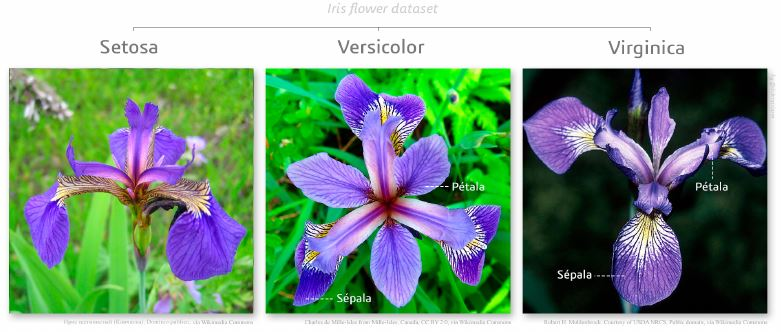
\includegraphics[width=\textwidth]{../figures/iris_species.jpg}

\vspace{0.3em}
{\small Three Iris flower species.}

\end{columns}
\end{frame}

%------------------------------------------------

\begin{frame}{Data: Iris Measurements}
\begin{columns}

\column{0.48\textwidth}

The four measured features can be used to classify flower species.

\vspace{0.5em}

Observations:
\begin{itemize}
\item Setosa is easily separated
\item Versicolor and Virginica overlap
\item Petal measurements provide better separation than sepal measurements
\end{itemize}

\vspace{0.5em}

Goal:
\begin{itemize}
\item Predict species from measurements
\end{itemize}

\column{0.52\textwidth}
\centering
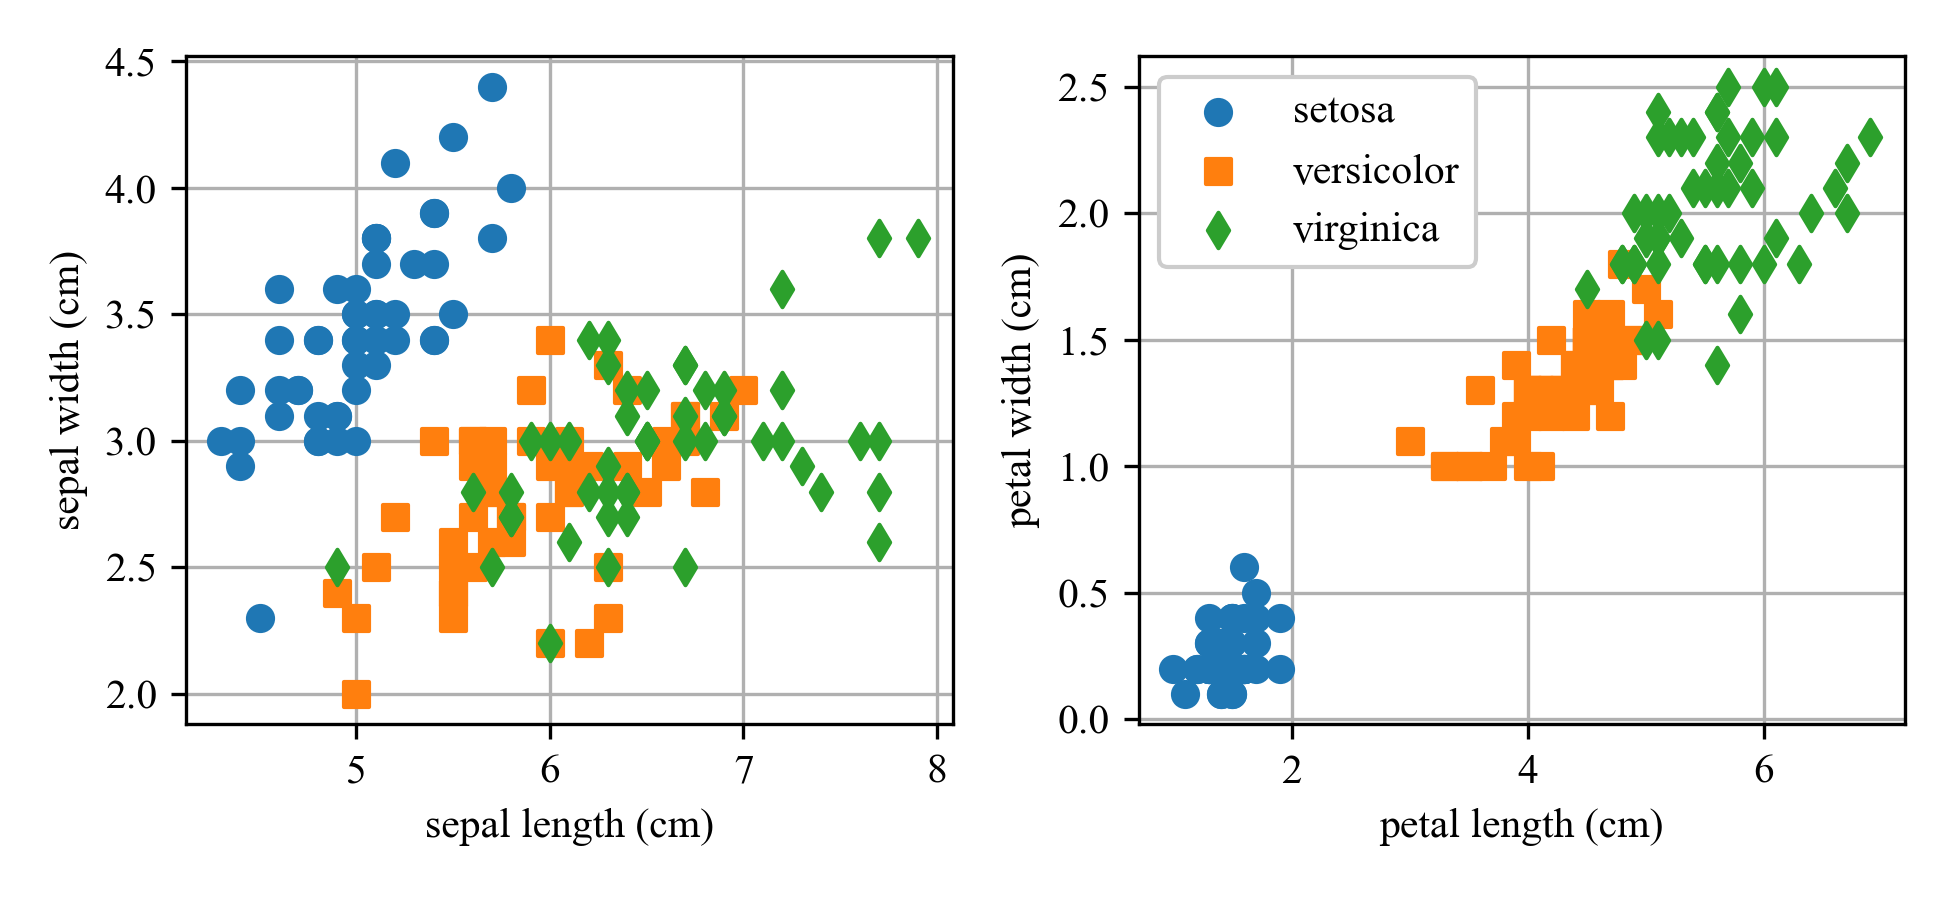
\includegraphics[width=\textwidth]{../figures/Iris_dataset_scatterplot.png}

\vspace{0.3em}
{\small Sepal and petal measurements for the Iris dataset.}

\end{columns}
\end{frame}

%------------------------------------------------

\begin{frame}{Example 5.1: Iris Dataset Exploration}

\begin{itemize}
\item Load the Iris dataset from Scikit-Learn
\item Examine feature and label information
\item Visualize sepal and petal measurements
\item Explore relationships between the three species
\end{itemize}

\vspace{0.5em}

Demonstrates:
\begin{itemize}
\item Classification datasets
\item Feature exploration
\item Data visualization
\item Class separation
\end{itemize}

\end{frame}

%------------------------------------------------

\begin{frame}{1-D Decision Boundaries}
\begin{columns}

\column{0.48\textwidth}

Logistic Regression can classify Iris-Virginica using a single feature:

\[
\text{Petal Width}
\]

\vspace{0.5em}

Observations:

\begin{itemize}
\item Below 1 cm:
\begin{itemize}
\item Confidently not Virginica
\end{itemize}

\vspace{0.3em}

\item Above 2 cm:
\begin{itemize}
\item Confidently Virginica
\end{itemize}

\vspace{0.3em}

\item Between:
\begin{itemize}
\item Model uncertainty
\end{itemize}
\end{itemize}

\column{0.52\textwidth}
\centering
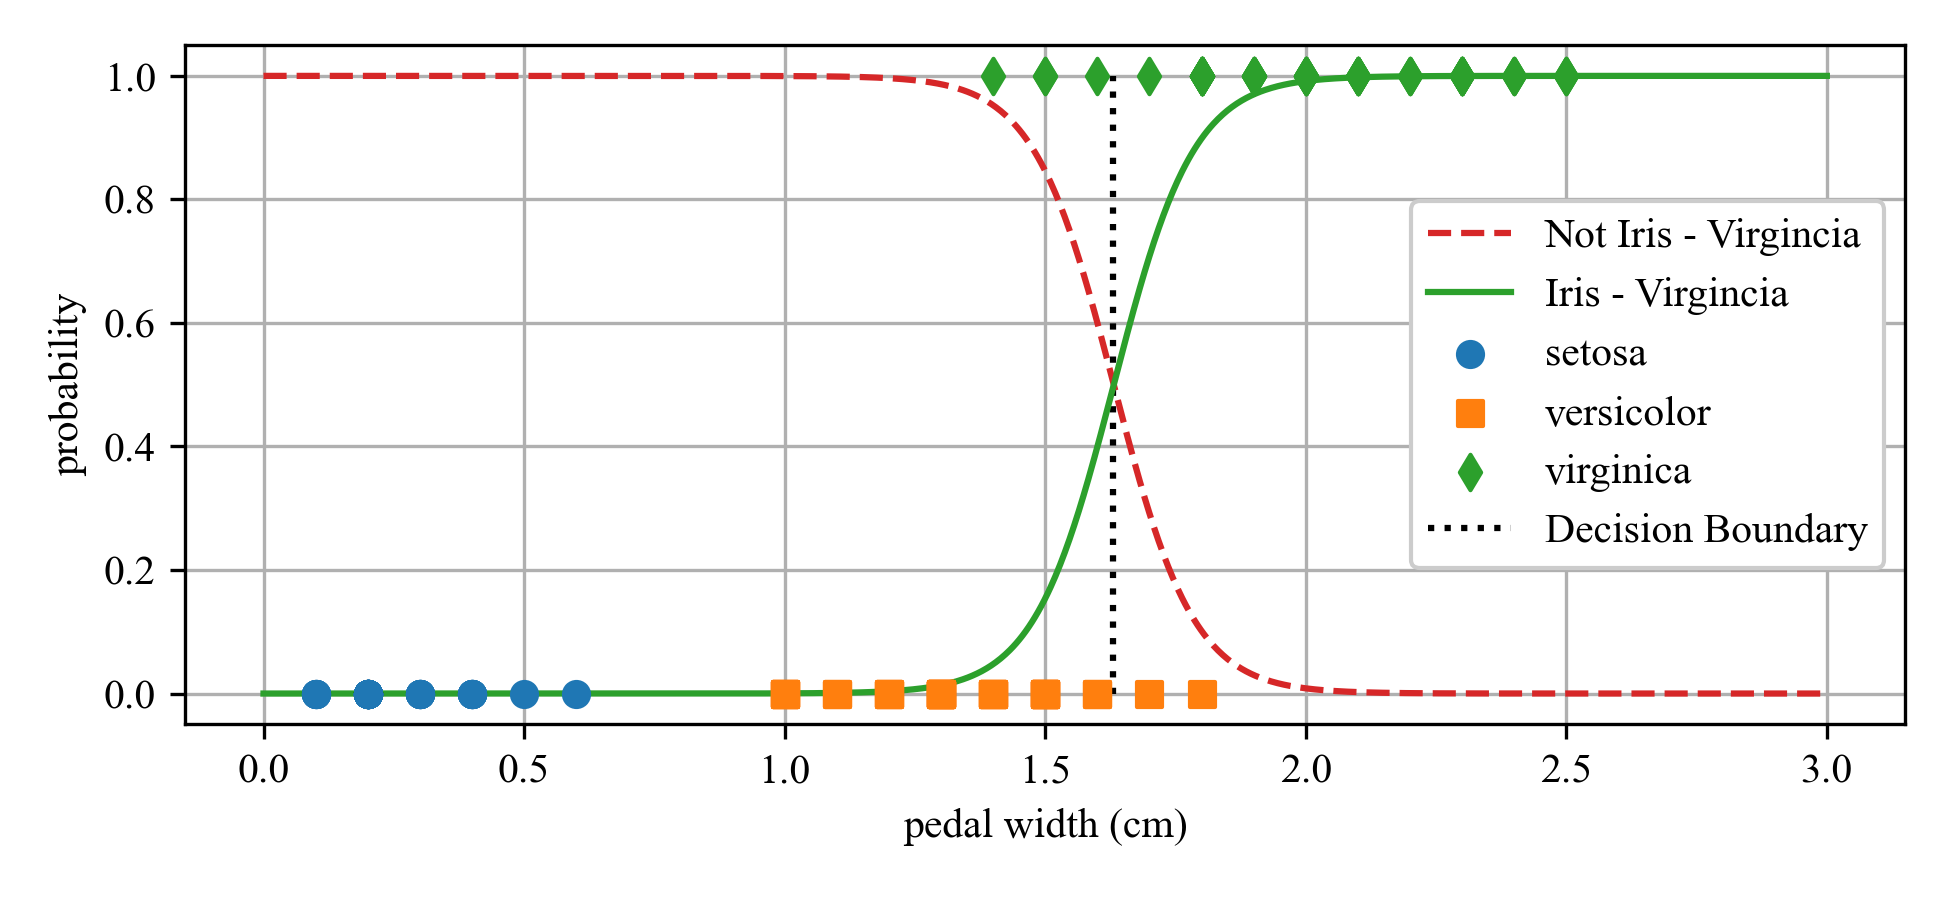
\includegraphics[width=\textwidth]
{../figures/Iris_dataset_decision_boundary_1D.png}

\vspace{0.3em}
{\small 1-D decision boundary.}

\end{columns}
\end{frame}

%------------------------------------------------

\begin{frame}{Decision Boundary}

A Logistic Regression model predicts probabilities:

\[
\hat{p}=P(y=1|X)
\]

\vspace{0.5em}

The classification boundary occurs when:

\[
\hat{p}=0.5
\]

\vspace{0.5em}

For the Iris dataset:

\begin{itemize}
\item Decision boundary occurs near:
\[
\text{Petal Width}\approx 1.6\text{ cm}
\]

\item Above the boundary:
\begin{itemize}
\item Predict Iris-Virginica
\end{itemize}

\item Below the boundary:
\begin{itemize}
\item Predict not Iris-Virginica
\end{itemize}
\end{itemize}

\end{frame}

%------------------------------------------------

\begin{frame}{Example 5.2: 1D Logistic Regression}

\begin{itemize}
\item Train a Logistic Regression model using:
\begin{itemize}
\item Petal width only
\end{itemize}

\vspace{0.5em}

\item Estimate:
\begin{itemize}
\item Probability of Iris-Virginica
\end{itemize}

\vspace{0.5em}

\item Visualize:
\begin{itemize}
\item Predicted probabilities
\item 50\% decision boundary
\end{itemize}

\vspace{0.5em}

\item Demonstrates how probabilities become class predictions
\end{itemize}

\end{frame}

%------------------------------------------------

\begin{frame}{2-D Decision Boundaries}
\begin{columns}

\column{0.48\textwidth}

Using two features:

\begin{itemize}
\item Petal length
\item Petal width
\end{itemize}

\vspace{0.5em}

The model predicts:

\[
P(\text{Virginica}|X)
\]

\vspace{0.5em}

Features:

\begin{itemize}
\item Dashed line:
\begin{itemize}
\item 50\% decision boundary
\end{itemize}

\item Contours:
\begin{itemize}
\item Equal probability levels
\end{itemize}

\item Upper-right region:
\begin{itemize}
\item High confidence Virginica
\end{itemize}
\end{itemize}

\column{0.52\textwidth}
\centering
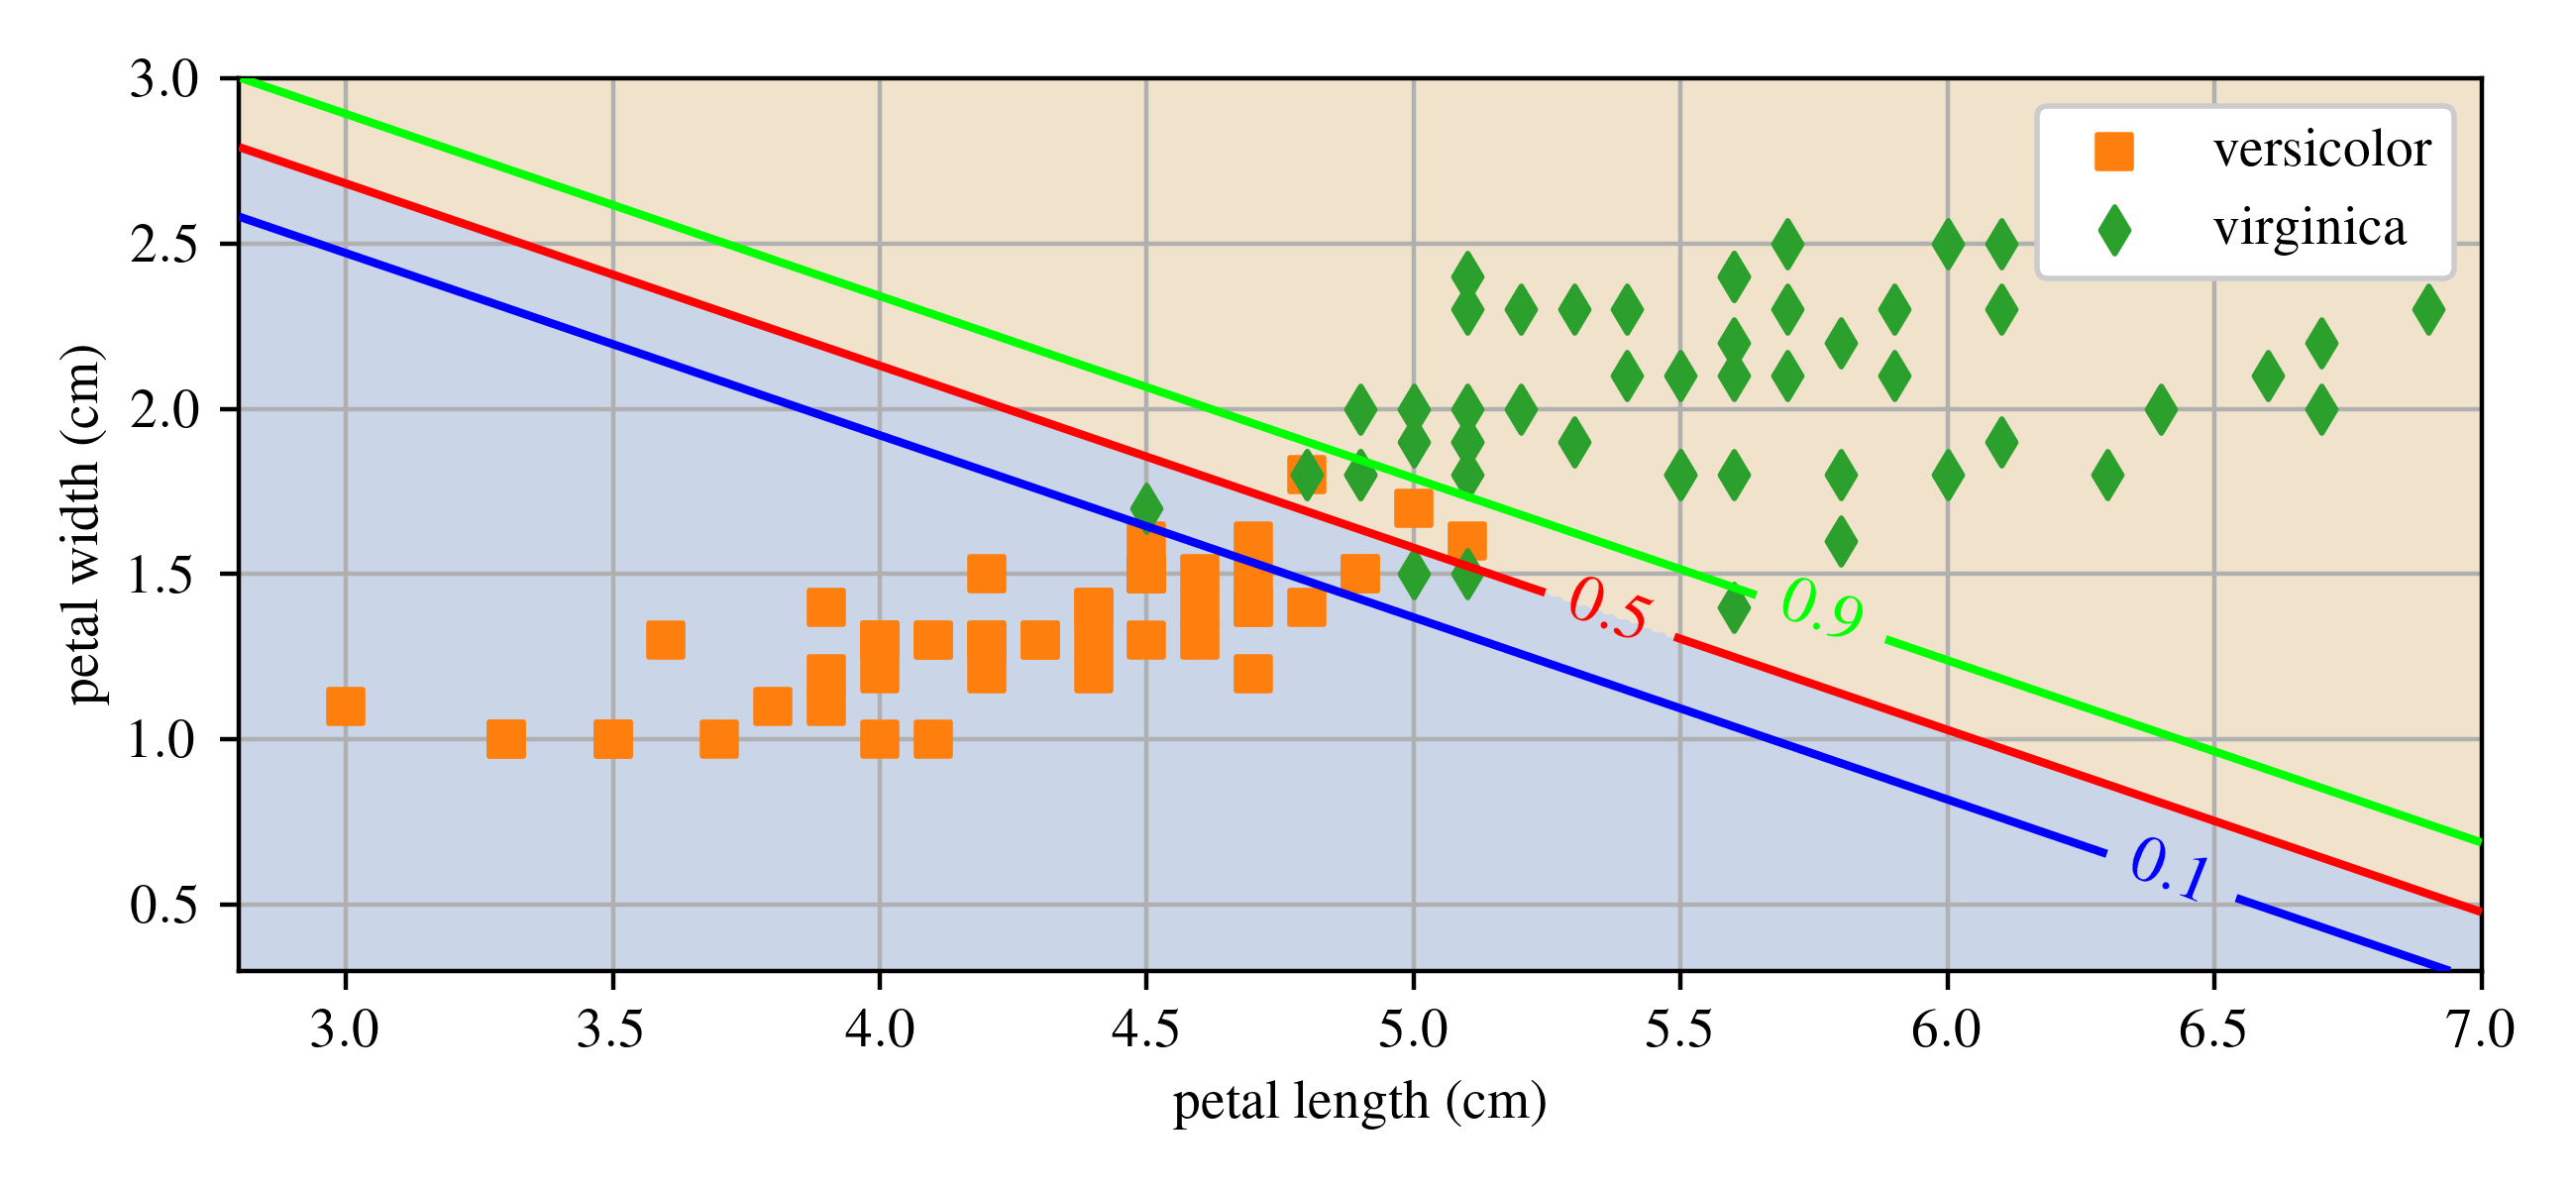
\includegraphics[width=\textwidth]
{../figures/Iris_dataset_decision_boundary_2D.png}

\vspace{0.3em}
{\small 2-D decision boundary and probability contours.}

\end{columns}
\end{frame}

%------------------------------------------------

\begin{frame}{Example 5.3: 2D Decision Boundary}

\begin{itemize}
\item Train a Logistic Regression model using:
\begin{itemize}
\item Petal length
\item Petal width
\end{itemize}

\vspace{0.5em}

\item Visualize:
\begin{itemize}
\item Classification regions
\item Decision boundary
\item Probability contours
\end{itemize}

\vspace{0.5em}

\item Demonstrates how Logistic Regression separates classes in a two-dimensional feature space
\end{itemize}

\end{frame}

%------------------------------------------------
\section{3.2~Softmax Regression}

\begin{frame}{Softmax Regression}
\begin{columns}

\column{0.48\textwidth}

Softmax Regression extends Logistic Regression to multiple classes.

\vspace{0.5em}

\begin{itemize}
\item No need to train several binary classifiers
\item Works when each input belongs to exactly one class
\item Also called Multinomial Logistic Regression
\end{itemize}

\vspace{0.5em}

For an input vector $\mathbf{x}$, the model computes a score for each class.

\vspace{0.5em}

Example:
\begin{itemize}
\item Classify all three Iris species simultaneously
\end{itemize}

\column{0.52\textwidth}
\centering
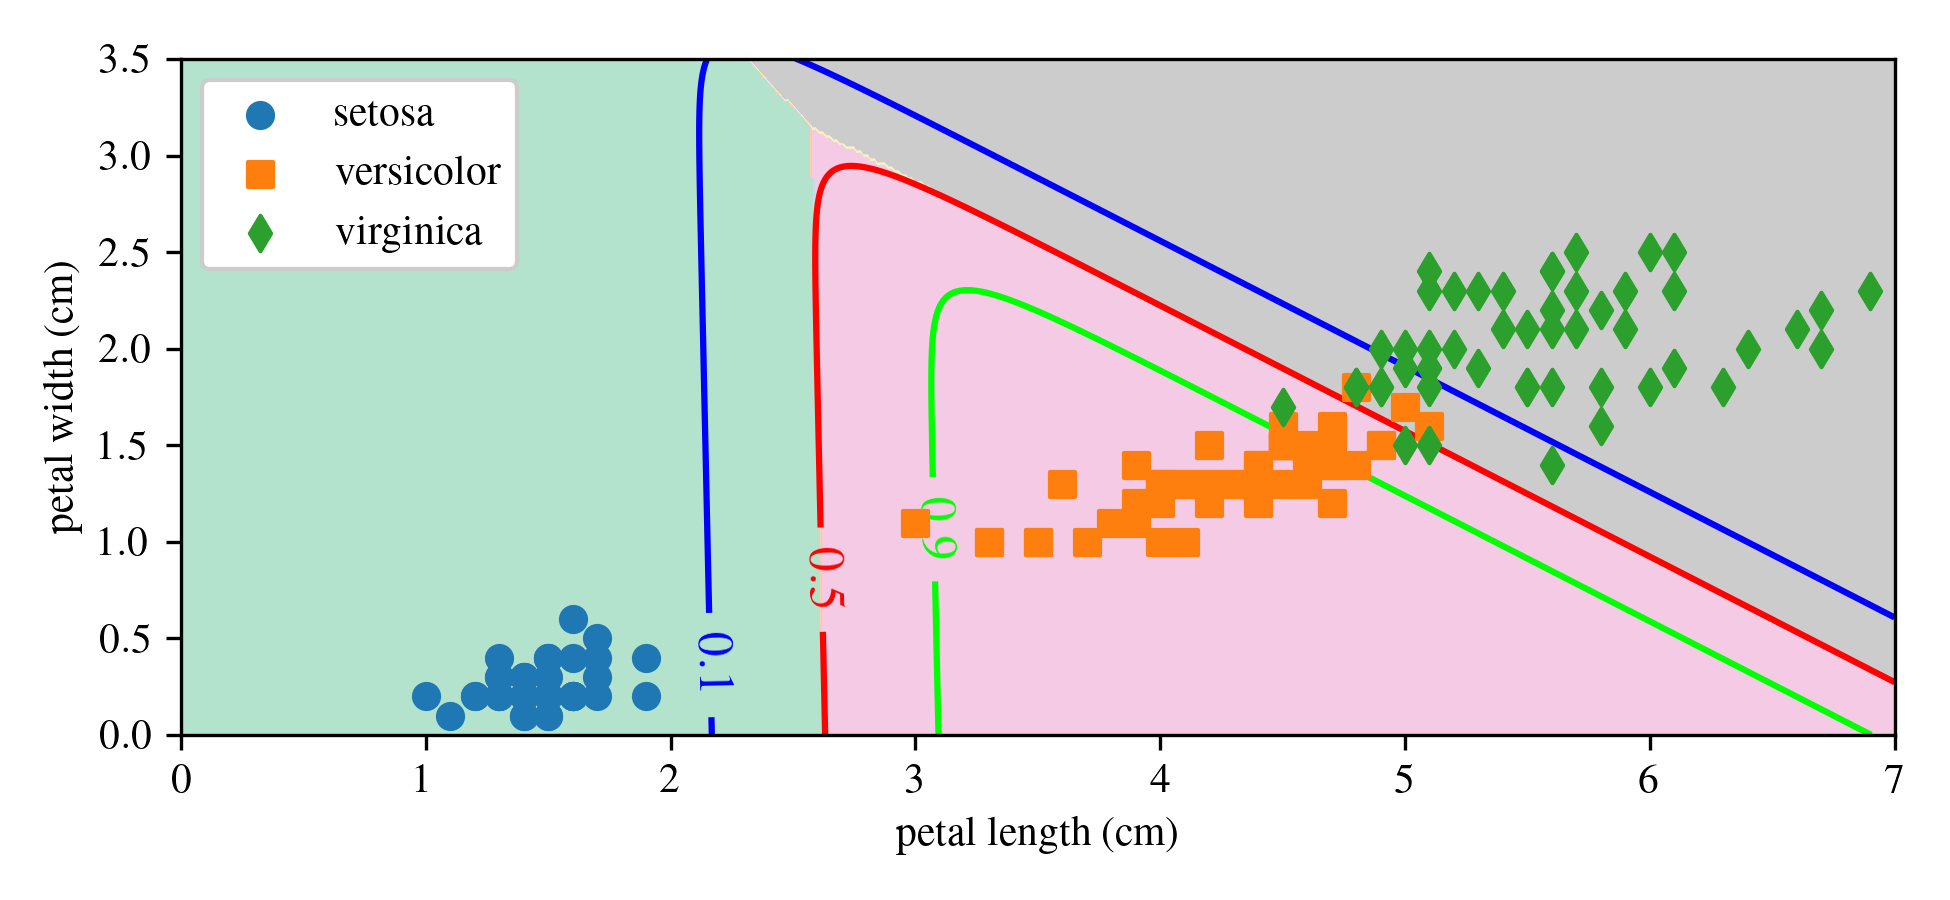
\includegraphics[width=\textwidth]
{../figures/Softmax_classification.png}

\vspace{0.3em}
{\small Softmax classification of the three Iris species.}

\end{columns}
\end{frame}

%------------------------------------------------

\begin{frame}{Class Scores and Probabilities}

For class $k$, the score is

\[
s_k(\mathbf{x}) = \mathbf{x}^{\top}\bm{\theta}^{(k)}
\]

\vspace{0.5em}

The softmax function converts scores into probabilities:

\[
\hat{p}_k
=
\frac{\exp\big(s_k(\mathbf{x})\big)}
{\sum_{j=1}^{K}\exp\big(s_j(\mathbf{x})\big)}
\]

\vspace{0.5em}

\begin{itemize}
\item $\mathbf{s}(\mathbf{x})$ is the vector of class scores
\item $K$ is the number of classes
\item All predicted probabilities sum to 1
\end{itemize}

\end{frame}

%------------------------------------------------

\begin{frame}{Prediction Rule}

Softmax Regression predicts the class with the largest probability:

\[
\hat{y}
=
\mathop{\mathrm{argmax}}_{k}\hat{p}_k
=
\mathop{\mathrm{argmax}}_{k}s_k(\mathbf{x})
=
\mathop{\mathrm{argmax}}_{k}\big((\bm{\theta}^{(k)})^{\top}\mathbf{x}\big)
\]

\vspace{0.5em}

\begin{exampleblock}{Note}
The argmax operator returns the index of the largest value.
\end{exampleblock}

\vspace{0.5em}

\begin{itemize}
\item Softmax Regression is multiclass, not multioutput
\item It predicts one class at a time
\item Useful for problems with mutually exclusive categories
\end{itemize}

\end{frame}

%------------------------------------------------

\begin{frame}{Training Softmax Regression}

The model is trained by minimizing the cross-entropy cost:

\[
J(\Theta)
=
-\frac{1}{m}
\sum_{i=1}^{m}
\sum_{k=1}^{K}
y_k^{(i)}\log\big(\hat{p}_k^{(i)}\big)
\]

\vspace{0.5em}

\begin{itemize}
\item Penalizes low probability for the true class
\item When $K=2$, this reduces to log loss
\item No closed-form solution
\item Train using Gradient Descent or another optimizer
\end{itemize}

\vspace{0.5em}

Gradient with respect to class $k$:

\[
\nabla_{\bm{\theta}^{(k)}}J(\Theta)
=
\frac{1}{m}
\sum_{i=1}^{m}
\big(\hat{p}_k^{(i)} - y_k^{(i)}\big)\mathbf{x}^{(i)}
\]

\end{frame}

%------------------------------------------------

\begin{frame}{Example 5.4: Softmax Classification}
\begin{columns}

\column{0.48\textwidth}

The Iris dataset can be classified using petal length and petal width.

\vspace{0.5em}

This example:
\begin{itemize}
\item Trains a multinomial logistic regression model
\item Uses \texttt{multi\_class="multinomial"}
\item Requires a solver such as \texttt{lbfgs}
\end{itemize}

\vspace{0.5em}

After training, a flower with 5 cm petals is classified as Iris-Virginica with probability 94.2\%.

\column{0.52\textwidth}
\centering
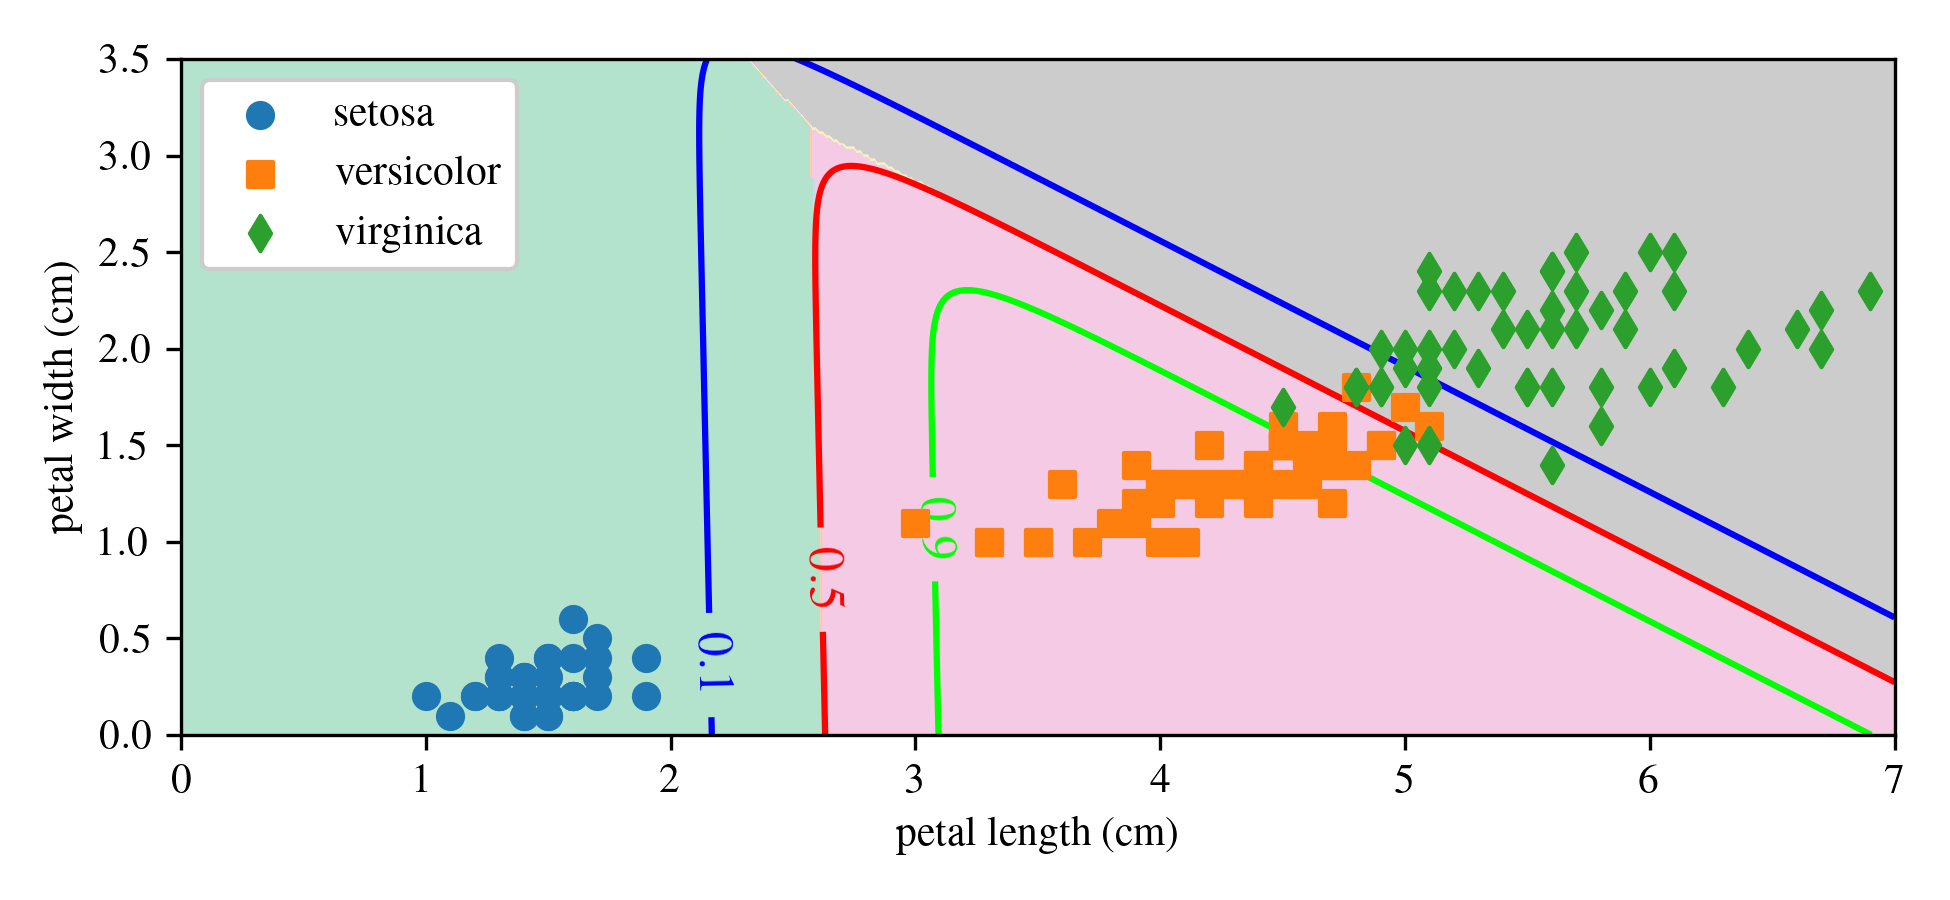
\includegraphics[width=\textwidth]{../figures/Softmax_classification.png}

\vspace{0.3em}
{\small Softmax classification for the three Iris species.}

\end{columns}
\end{frame}


























\end{document}




